\documentclass[class=book, crop=false]{standalone}
\usepackage[utf8]{inputenc}
\usepackage[subpreambles=true]{standalone}
\usepackage{import}
\usepackage[ruled,vlined]{algorithm2e}

\usepackage{amsmath}
\usepackage{amssymb}
\usepackage[margin=1.2in]{geometry}
\usepackage[sorting = none,
            doi = true  %lesedato for url-adresse
            ]{biblatex} %none gir bibliografi i sitert rekkefølge
\addbibresource{reference.bib}
\usepackage{csquotes}
\usepackage{pgfplots}
\usepackage{pgfplotstable}

\pgfplotsset{compat=1.15}

\begin{document}
\chapter{Results}\label{chapter:results}

There are many ways of setting up the state space and reward function that can result in very different behaviour of the agent. This chapter will present results from certain formulations of the reinforcement algorithm. In all cases, deep deterministic policy gradient (DDPG) is used to train the agent. 

\section{Feasibility}
It is important to investigate the potential effect demand response have before a model is evaluated. It is not given that it is physically feasible avoid safety violation in critical periods for a given flexibility. Therefore, it is necessary to discuss the physical challenges in the electrical grid, and the kind of behaviour that would improve the situation. As mentioned in \ref{chap:problem_description}, the main challenges for the network is that large amount of power must imported and exported out to the external grid in a normal day. Figure \ref{fig:results:demand_and_solar} plots the daily mean solar irradiance signal and power demand used for training the reinforcement agent. The first period that is critical for the grid is when the solar irradiance is at its maximum. The excess solar power produced must be transported out to the grid through many lines due to a large amount of local power production. This can cause overloads in the lines carrying the current and high voltage magnitudes at the bus bars. The second critical period is during peak demand because large amount of energy must be imported from the grid. The problem with importing large amounts of power is potential overloads in the lines, in addition to low voltage magnitudes. A solution to this problem is that profile for the solar production and power demand overlap more. It is not possible to control when the sun shines, but it is possible to manipulate when power is consumed.
\begin{figure}[h]
    \center
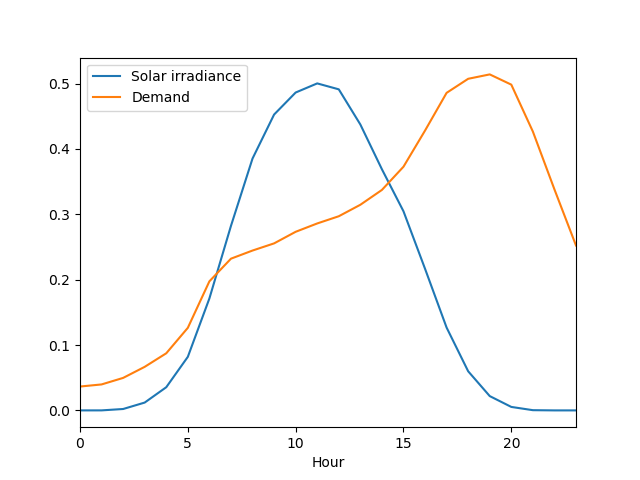
\includegraphics[height=8cm, width=12cm]{figures/demand_and_solar.png}
    \caption[size = 9]{Mean hourly power demand curve and solar irradiance}
    \label{fig:results:demand_and_solar}
\end{figure}

The reinforcement agent is trained with a certain flexibility. It is necessary to inspect what effect the activation of flexibility has on voltage magnitude and line current before a trained agent can be evaluated. Figure \ref{fig:results:increase_demand_current} illustrates the effect activation of flexibility (increasing consumption) has on the current in a critical line. The consumption of active power is increased by 25 \% for all the loads in every hour. The first and second peak in plot correspond, respectively, to the solar peak and the power demand peak. It is clear from the first peak that increasing the consumption decreases the line current. This is because the loads in this period generate so much solar power that they act as producers and not consumers. Increasing the consumption means that less power needs to be transported out to the external grid, which decreases the line current. As a result, the desired behaviour in periods with high solar irradiation is to increase the consumption.


\begin{figure}[h]
    \center
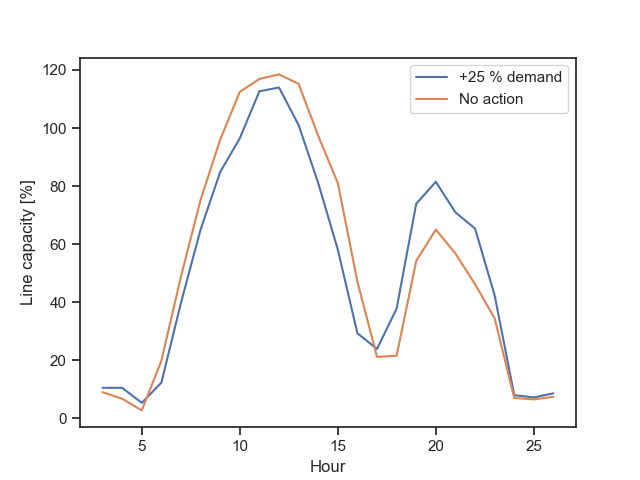
\includegraphics[height=8cm, width=12cm]{figures/increase_demand_current.png}
    \caption[size = 9]{Current capacity in a critical line when increasing the power consumption with 25 \% in all hours and regular situation. The line connecting bus 1 and 2 in figure \ref{fig:problem:cigre_network} is showed}
    \label{fig:results:increase_demand_current}
\end{figure}

The effect of increasing consumption in the second peak is the opposite of that in the first peak. This is because the loads now act as consumers since there is no solar production. The active power must therefore be imported from the external grid. Increasing the consumption in this period simply corresponds to drawing even more power from the external grid, which in turn increases the line current. The desired behaviour in this period is therefore to lower the power consumption, since this would decrease the current in the line. 

\begin{figure}[h]
    \center
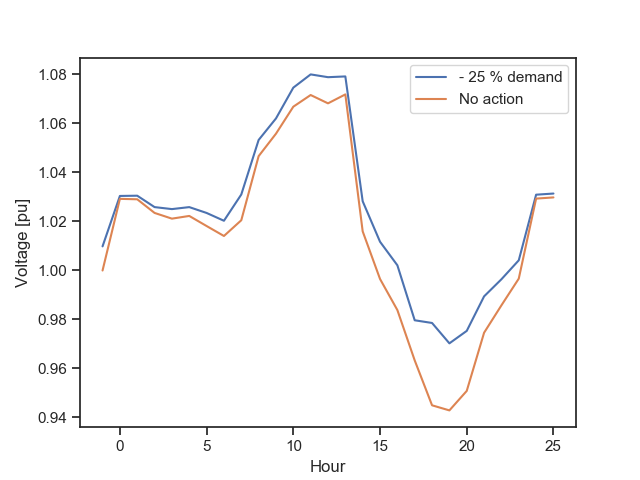
\includegraphics[height=8cm, width=12cm]{figures/decrease_demand_voltage.png}
    \caption[size = 9]{Voltage magnitude at critical bus when the power consumption is reduced with 25 \% in all hours and regular situation. Bus bar 9 in \ref{fig:problem:cigre_network} is used}
    \label{fig:results:decrease_demand_voltage}
\end{figure}

Figure \ref{fig:results:decrease_demand_voltage} illustrates the effect activation of flexibility has on voltage magnitude at a critical bus bar. In this case, the consumption of active power is decreased by 25 \% at all loads in the network. There are two critical periods during a normal day for this case as well. The effect of decreasing the consumption in periods with high solar is that the voltage magnitude increases. This can be seen between around hour 13 in figure \ref{fig:results:decrease_demand_voltage}. The bus bar is in this period acting as a producer because of the excess solar power that is transported out to the external grid. Generally, higher production at a bus bar means higher voltage magnitude. Reducing the consumption means that even more power from solar production must be sent out to the external grid, raising the voltage magnitude ever further. Consequently, decreasing the consumption in periods with high solar irradiance is not a desired behaviour. 


The second critical period in a normal day can be seen around hour 20 in figure \ref{fig:results:decrease_demand_voltage}. At this point, there is no solar power production, and power must be imported from the external grid. The voltage magnitude is now lower than its nominal value because the loads consume. Generally, higher consumption means lower voltage magnitude. Therefore it is better to reduce the consumption of power in this period because the voltage magnitudes will be closer to nominal values.

The desired behaviour in terms of both current and voltage safety margins is to increase consumption in periods with high solar irradiance and decrease it when the production of solar energy has ended.


\section{Formulation 1 - Free activation} \label{section:result:config1}
A reinforcement agent is trained with reward function that does not include cost of activation. This is not a realistic case, since households that offer flexibility should be compensated for altering their energy profile. This formulation serves to show how an agent would activate flexibility if there was no direct cost associated with altering the power consumption. However, the agent is penalised for changing the total daily energy demand in the power net. Note that it is not penalised for changing the daily consumption at individual loads as long as the total consumption in the network is preserved. The specific reward terms with weights are shown in table \ref{table:results:reward_formulation1}

\begin{table}[h]
\centering
\begin{tabular}{l|ll}

Cost  & Weight & Comment
\\ 
\hline
Voltage &
1 &
Per-unit values
\\
Current &
$10^{-2}$ &
Percentage of max current 
\\
Activation &
0&
No activation cost
\\
Imbalance &
$10^{-4}$&
Units of energy imbalance is kWh
\\
\hline
\end{tabular}
\caption{Reward terms and weights for formulation 1}
\label{table:results:reward_formulation1}
\end{table}
The state space is constructed to be as small as possible. The state is represented by a 4 hour forecast for both solar irradiance and active power demand. The power demand is assumed equal at each flexible load, so there is not an individual power demand for each load. The total power imbalance for the whole power network is also included. Table \ref{table:results:state_formulation1} summarises the state space

\begin{table}[h]
\centering
\begin{tabular}{l|lll}

State space  & Size & Comment
\\ 
\hline
Solar forecast      &  4  &  4 hour solar forecast
\\ 

Demand forecast    &4 & One 4 hour forecast for all loads
\\ 
Imbalance state & 1  & Total energy imbalance for all loads
\\
\hline
\end{tabular}
\caption{State used in formulation 1}
\label{table:results:state_formulation1}
\end{table}


\begin{figure}[h]
    \center
    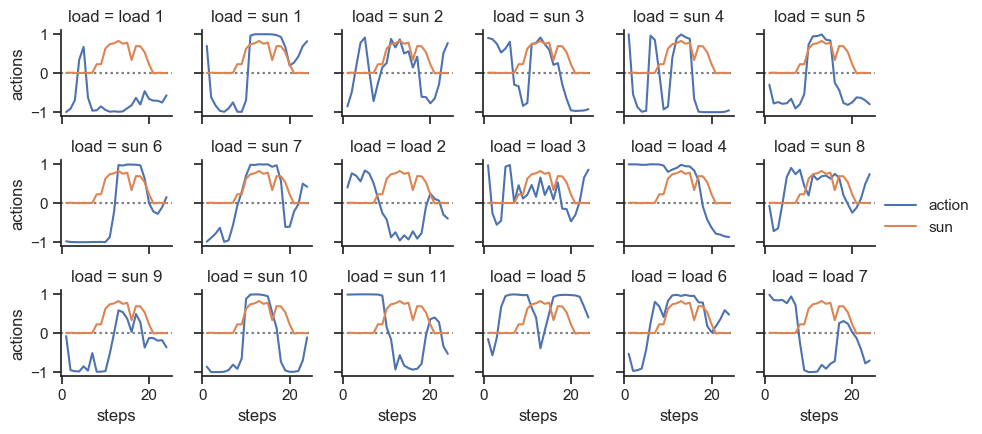
\includegraphics[scale=0.7]{figures/configuration1.png}
    \caption[size = 9]{Activation of flexibility at the different flexible loads of the trained agent throughout a day. The line line is the solar irradiance during the day, which is the same for all loads. The actions in green is the activation of flexibility. Action = 1 means that the flexible load increases its power consumption with 10 \%, while action = -1 means that it decreases its power consumption with 10 \%}
    \label{fig:results:configuration1}
\end{figure}

The DDPG agent was trained for 100 000 time steps. A complete summary with all hyper-parameters used can be found in appendix \ref{section:apendix_config1}. Figure \ref{fig:results:configuration1} visualises the actions of the trained agent throughout a day (24 hours) together with the solar irradiance. Because the solar power production in the system is very large, the safety margins for current and voltage are frequently violated. The desired behaviour of the agent is therefore to increase consumption in periods with high solar irradiance, and decrease it during peak demand in the afternoon. This helps the system because the power is not transported out to the grid, but instead is consumed locally. Simply put, it is desired that the actions follow the curve of the solar irradiance around noon, and goes down in the afternoon. 

\begin{figure}[h]
    \center
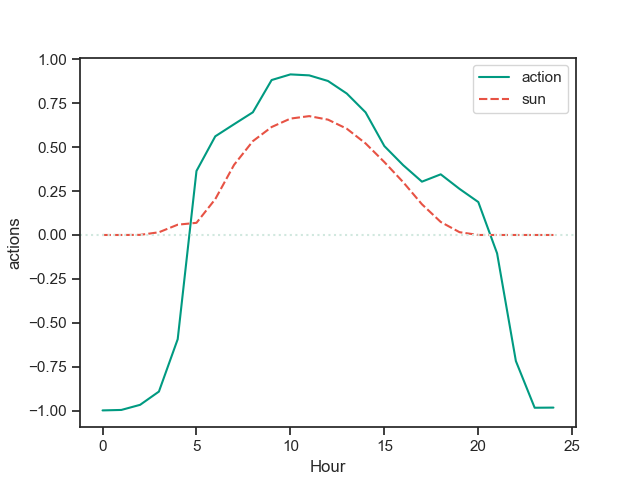
\includegraphics[scale=0.7]{figures/configuration1_follows_sun.png}
    \caption[size = 9]{Action of the agent and solar profile during a day. The consumed power is increased in periods with high solar production}
    \label{fig:results:configuration1_follows_sun}
\end{figure}

By inspecting figure \ref{fig:results:configuration1} it is clear that the agent activates flexibility in times with much solar production for several of the loads. The plot \texttt{load = 12} in is shown alone in figure \ref{fig:results:configuration1_follows_sun}, and clearly follows this pattern. The agent increases its power consumption during periods with high solar production, and reduces it later during peak demand.


\begin{figure}[h]
    \center
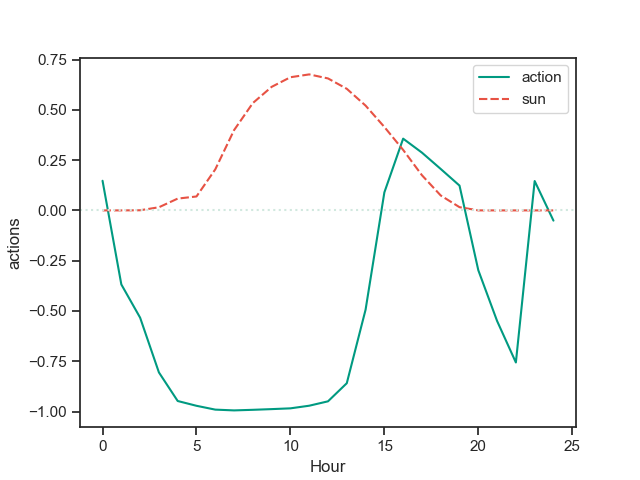
\includegraphics[height=8cm, width=12cm]{figures/configuration1_negative_actions.png}
    \caption[size = 9]{Action of the agent and solar profile during a day}
    \label{fig:results:configuration1_negative_actions}
\end{figure}

The plot \texttt{load 8} is shown alone in figure \ref{fig:results:configuration1_negative_actions}, and show some peculiar behaviour. Clearly, the actions do not follow the solar profile that day, but are negative most of the day. This behaviour could be a result of how the reward function is defined in this configuration. The agent is penalised according to the total energy imbalance in the system, not at individual loads. As a result, if the energy imbalance is +1 MWh at one load and -1 MWh at another load, they perfectly cancel each other, and the agent is not penalised. From the agent's perspective, the system is in energy balance, although individual loads may have a large absolute energy imbalance. This illustrates the problem with constructing state variable that accounts for the system as a whole, and not individual loads. The agent uses the same strategy consistently at this load. It appears as if this load functions as an energy balance, whose main job is to ensure that the total power imbalance in the grid is kept as small as possible. However, the behaviour of the agent gives a negative energy imbalance in the long term, as seen in figure \ref{fig:results:configuration1_energy_imbalance}. The agent controls a 200 hour long episode, and it is evident that the energy imbalance quickly decreases and reaches an equilibrium around -13 MWh. The agent prefers to decrease the total consumption in the system. It may indicate that the reward function is not appropriately constructed. More specifically, the energy imbalance cost is designed to reward the agent every time the energy imbalance decreases in absolute magnitude. A problem with this approach could be that the agent is not penalised for having a large absolute power imbalance. The reward function considers an energy imbalance transition from -11 MWh to -10 MWh equally good as a transition from -1 MWh to 0 MWh.
 
\begin{figure}[H]
    \center
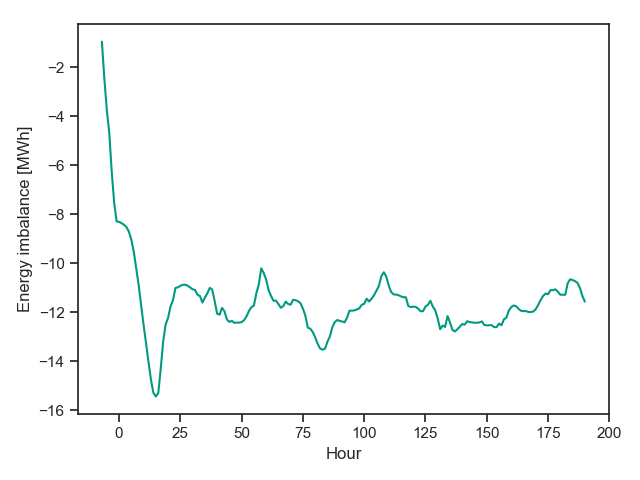
\includegraphics[height=8cm, width=12cm]{figures/configuration1_imbalance.png}
    \caption[size = 9]{Total energy imbalance in the system during a 200 hour episode controlled by the trained agent}
    \label{fig:results:configuration1_energy_imbalance}
\end{figure}

\subsection{Voltage violations}
The reward function has an energy imbalance term during training that is meant to incentives the agent to shift energy consumption. However, the main goal of the agent is to keep the values for current and voltage within safety margins. Therefore, it is interesting to see the rewards of the trained model when only the voltage and current terms are considered. In other words, the agent is only penalised for violating safety margins for current and voltage in the grid. The trained model was tested for 500 episodes each consisting of 200 steps and evaluated
in terms of voltage penalty and current penalty independently. The statistics for the hours with a non-zero reward using only voltage reward are presented in table \ref{table:results:configuration1_reward_500_episodes}. Note that every non-zero reward corresponds to a violation of voltage margin because only the voltage term is used to calculate the reward. The trained agent reduces the number of voltage safety margin violations by 13 \% from 8593 to 7484. This reduction is impressive since there is no guarantee that it is physically feasible to satisfy voltage safety margins given a demand flexibility of 10 \%. It is clear that there is no significant difference between the trained agent and the no agent scenario in terms of mean voltage reward. Still, the reduction in number of voltage violations means that the trained agent overall is performing better in the 500 episodes. 
\begin{table}[h]
\center
\begin{tabular}{l|rrrrrrr}
         & count & mean   & std   & min    & 25\%   & 50\%   & 75\%   \\
\hline
Agent    & 7484  & -0.033 & 0.035 & -0.189 & -0.049 & -0.021 & -0.007 \\
No agent & 8593  & -0.035 & 0.037 & -0.186 & -0.054 & -0.022 & -0.006 \\
\hline
\end{tabular}
\caption{Statistics of the voltage rewards given to the trained agent and no agent scenario over 500 episodes with 200 hours each}
\label{table:results:configuration1_reward_500_episodes}
\end{table}

Figure \ref{fig:results:config1_voltage_boxplot} shows the voltage reward distribution for the trained agent and no agent scenario for hours with violations of voltage safety margins. These hours are termed critical since there would be voltage violations if no actions were taken. The trained agent is better in critical situations, as more of the rewards are centred closer to zero.

\begin{figure}[H]
    \center
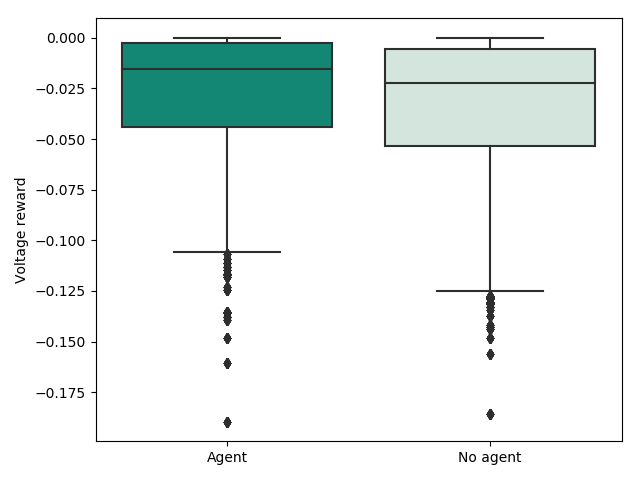
\includegraphics[height=8cm, width=12cm]{figures/config1_voltage_boxplot.png}
    \caption[size = 9]{Box plot of the reward distribution of the trained agent and no agent scenario for critical hours where safety margins are violated.}
    \label{fig:results:config1_voltage_boxplot}
\end{figure}

The statistics presented in table \ref{table:results:configuration1_reward_500_ep_preventive} show that the mean voltage penalty for the trained agent is reduced by 17 \% in critical hours. However, as table
\ref{table:results:configuration1_reward_500_episodes} shows, the average voltage penalty of the trained agent is about the same as the no agent scenario. This means that there are situations where the trained agent pushes the voltage out of the safety margins.    


\begin{table}[h]
\center
\begin{tabular}{l|rrrrrrr}
         & count & mean   & std   & min    & 25\%   & 50\%   & 75\%   \\
\hline
Agent    & 8593 & -0.029 & 0.034 & -0.190 & -0.044 & -0.015 & -0.003 \\
No agent & 8593 & -0.035 & 0.037 & -0.186 & -0.054 & -0.022 & -0.006 \\
\hline
\end{tabular}
\caption{Statistics of the voltage rewards given in critical hours to the trained agent and no agent scenario over a 500 episodes simulation with 200 hours each}
\label{table:results:configuration1_reward_500_ep_preventive}
\end{table}



All rewards in the no agent scenario for critical hours are sorted and plotted in figure \ref{fig:results:config1_sorted_voltage}. The corresponding rewards given to the trained agent are also plotted. This is done to see if the trained agent is better in very critical periods with high voltage penalty or if it performs well overall. The plot shows that the trained agent for the most part receives lower voltage penalties regardless of the size of the violation. Still, there are occasions where the trained agent is below the no agent scenario in figure \ref{fig:results:config1_sorted_voltage} which corresponds to periods where the trained agent aggravates the voltage magnitudes. The trained agent makes matters worse in 41\% of the critical hours, and increases the mean penalty with 13 \% in those hours. However, the trained agent improves the voltage margins in 59 \% of the critical hours, where it decreases the mean voltage penalty by 38 \%.



\begin{figure}[h]
    \center
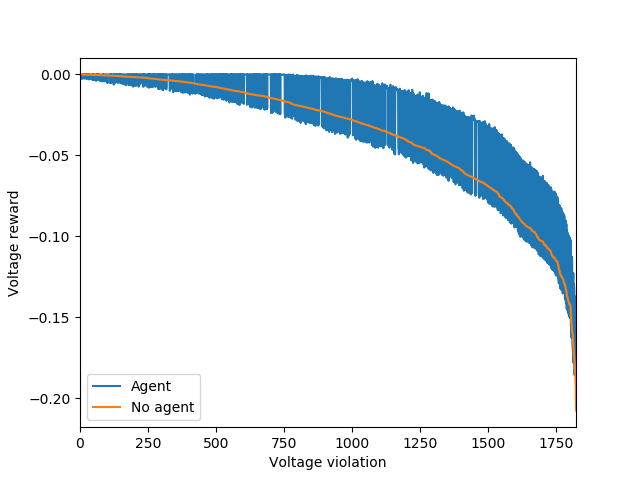
\includegraphics[height=8cm, width=12cm]{figures/config1_sorted_voltage.png}
    \caption[size = 9]{Voltage rewards given to the trained agent and no agent scenario in critical hours. The rewards are sorted for the no agent scenario from best to worst}
    \label{fig:results:config1_sorted_voltage}
\end{figure}


Figure \ref{fig:results:config1_improvement_voltage} shows for each hour of a day a box plot of difference between the voltage reward given to the trained agent and no agent scenario in critical hours. This plot illustrates the improvements of the trained agent, measured in terms of the increase in voltage reward. It is clear that the trained agent only is better in the afternoon, in periods of peak demand. 

\begin{figure}[h]
    \center
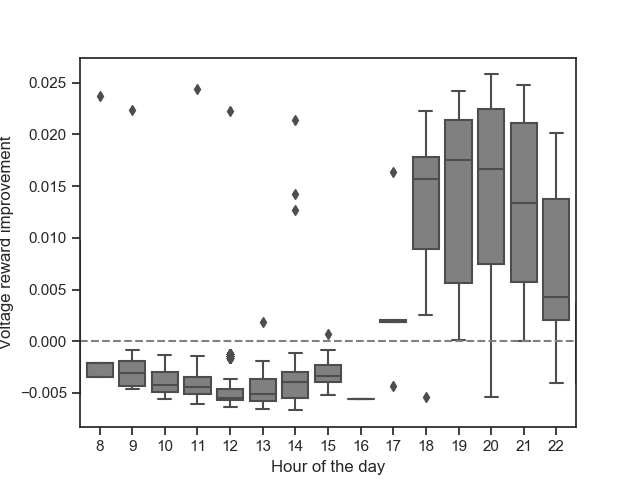
\includegraphics[height=8cm, width=12cm]{figures/config1_improvement_voltage.png}
    \caption[size = 9]{Hourly box plots of the difference in voltage rewards between the trained agent and no agent scenario in critical hours. Positive values means that the trained agent is better}
    \label{fig:results:config1_improvement_voltage}
\end{figure}


Figure \ref{fig:results:config1_400hour_good_voltage} plots the voltage rewards in a 400 hour episode for the trained agent and for a no-agent. This is period where the agent behaves well and reduces the number of violations of voltage safety margins. 

\begin{figure}[H]
    \center
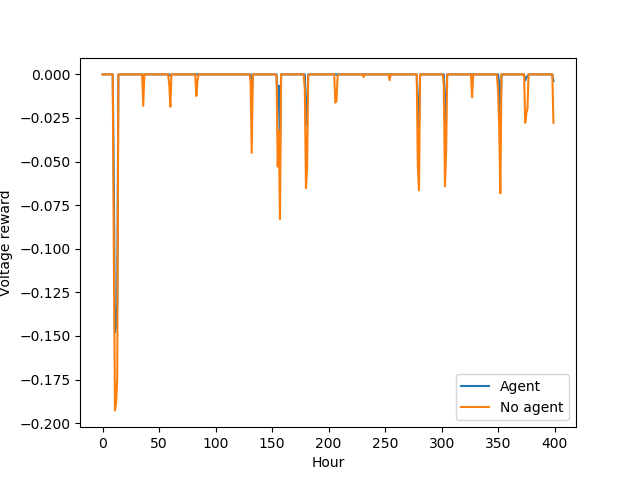
\includegraphics[height=8cm, width=12cm]{figures/config1_400hour_good_voltage.png}
    \caption[size = 9]{Voltage reward given to the trained agent and no agent scenario in a 400 hour episode}
    \label{fig:results:config1_400hour_good_voltage}
\end{figure}


The rewards are zero for the most part because the safety margins are generally satisfied. It is clear that in the episode the trained agent has learned a strategy that pulls voltage values close to nominal values. Table \ref{table:results:config1_400hour_good_voltage} shows statistics for when the trained agent and no-agent scenario violate voltage safety margins (non-zero reward). The trained agent reduces the number of violations from 37 to 23, a decrease of 38 \%.  In addition, the mean voltage penalty is 21 \% lower for the trained agent in the critical hours. Inspecting the rewards from the 400 episode shown in figure \ref{fig:results:config1_400hour_good_voltage} reveals that the agent in all cases prevents violation of voltage margins in peak demand periods. Consequently, the trained agent has learned a desired behaviour that decreases the peak power demand and thus keeps the voltage magnitude above the lower safety margin.

\begin{table}[h]
\center
\begin{tabular}{l|rrrrrrr}
         & count  & mean   & std   & min    & 25\%   & 50\%   & 75\%   \\
\hline
Agent    & 23 & -0.033 & 0.046 & -0.148 & -0.031 & -0.019 & -0.004 \\
No agent & 37 & -0.042 & 0.050 & -0.193 & -0.054 & -0.022 & -0.009 \\
\hline
\end{tabular}
\caption{Statistics of the rewards given to the trained agent and no agent scenario in a 400 hour episode when the trained agent behaves well}
\label{table:results:config1_400hour_good_voltage}
\end{table}

Figure \ref{fig:results:config1_150hour_bad_voltage} plots the voltage rewards in a 150 hour episode where the trained agent behaves poorly. The trained agent makes matter worse in most cases.

\begin{figure}[H]
    \center
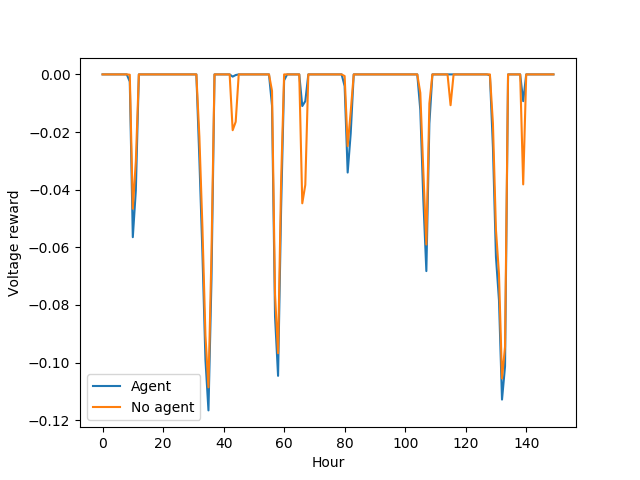
\includegraphics[height=8cm, width=12cm]{figures/config1_150hour_bad_voltage.png}
    \caption[size = 9]{Voltage rewards in a period the trained agent behaves badly and aggravates the situation}
    \label{fig:results:config1_150hour_bad_voltage}
\end{figure}
Table \ref{table:results:config1_150hour_bad_voltage} shows the statistics for the hours the trained agent and no-agent scenario violate voltage safety margins (non-zero rewards). The trained agent increase the number of voltage violation from 30 to 31. All of the hours the trained agent is worse in figure \ref{fig:results:config1_150hour_bad_voltage} correspond to hours of peak solar production. The spikes where it improves the situation correspond to periods with peak demand. As already mentioned, the trained agent has learned that it must decrease consumption in periods peak demand hours. On the contrary, it has not learned that it has to increase consumption in hours with heavy solar power production. In fact, it decreases the power consumption, which in turn makes the excess solar production even greater and thus increases voltage magnitudes in the grid.  

Until now, the the trained agent has been evaluated in critical hours, where there would be a safety violation in the no agent scenario. However, the electric grid is within safety margins 91 \% of the time in the 500 episode simulation. It is very important that the trained agent finds appropriate behaviour in both non-critical and critical hours. Investigating the voltage penalty given to the agent in non-critical hours reveals that the agent pushes the voltages out of the safety margins 0.3 \% of the time. The worst of these violations is -0.0007 in magnitude, which is negligible  compared the violations in critical hours. In other words, the agent behaves well in non-critical hours in terms of voltage. 
\begin{table}[h]
\center
\begin{tabular}{l|rrrrrrr}
         & count  & mean   & std   & min    & 25\%   & 50\%   & 75\%   \\
\hline
Agent    & 31    & -0.043 & 0.038 & -0.117 & -0.070 & -0.034 & -0.010 \\
No agent & 30    & -0.043 & 0.033 & -0.109 & -0.061 & -0.038 & -0.017 \\
\hline
\end{tabular}
\caption{Statistics of the rewards given to the trained agent and no agent scenario in a 150 hour episode when the trained agent behaves poorly}
\label{table:results:config1_150hour_bad_voltage}
\end{table}




\subsection{Current violations}\label{section:config1:current_violations}
The trained agent is tested in a 500 episode simulation, each consisting of 200 hours, and evaluated in terms of violations of current safety margins in the power lines. Specifically, the current cost $C_{current}$ for a line carrying a current $I$ with capacity $I_{max}$ is $C_{current} = \max(0,I - I_{max})$ where $I_{max}$ is set to 90 \% of the line capacity. The total current cost is found by summing over all lines. Note that the terms \textit{cost} and \textit{reward} are used interchangeably, depending on what is most natural. In all cases the reward is the negative of the cost. The statistics for the current violation for the trained agent and no agent scenario are presented in table \ref{table:results:configuration1_reward_500_episodes_current}

\begin{table}[h]
\center
\begin{tabular}{l|rrrrrrr}
         & count & mean   & std   & min    & 25\%   & 50\%   & 75\%   \\
\hline
Agent    & 1538  & -0.167 & 0.141 & -0.585 & -0.258 & -0.129 & -0.054 \\
No agent & 1300  & -0.168 & 0.135 & -0.564 & -0.257 & -0.156 & -0.045 \\
\hline
\end{tabular}
\caption{Statistics of the current rewards given to the trained agent and no agent scenario over a 500 episodes simulation, each with a duration of 200 hours}
\label{table:results:configuration1_reward_500_episodes_current}
\end{table}
The trained agent increases the number of current violations by 18 \% from 1300 to 1538. The mean magnitude of current violation is around the same in both scenarios. The agent has not learned an appropriate behaviour to reduce current overloads in the lines. The hours in the simulation that have a current violation if no action is taken are termed critical hours. Figure \ref{fig:results:config1_current_boxplot} shows the distribution of the current reward for the trained agent and no agent scenario in critical hours. 

\begin{figure}[H]
    \center
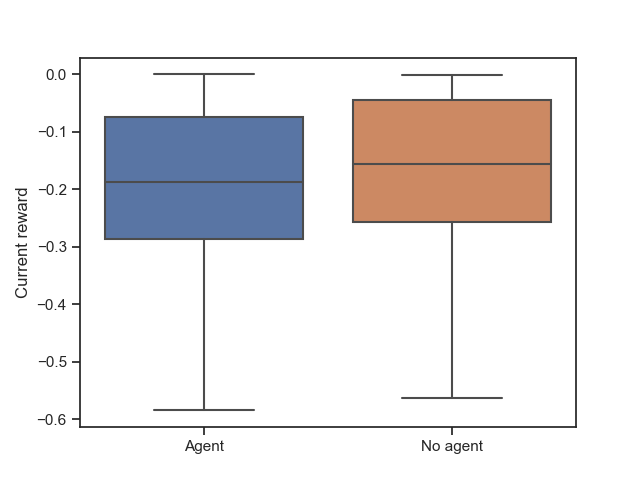
\includegraphics[height=8cm, width=12cm]{figures/config1_current_boxplot.png}
    \caption[size = 9]{Box plot of the current reward for the trained agent and no agent scenario}
    \label{fig:results:config1_current_boxplot}
\end{figure}
Figure \ref{fig:results:config1_sorted_current} plots the current reward for critical hours in the 500 episode sorted from best to worse. The hour with the lowest current reward is the most critical hour. It is clear that the trained agent for the most part aggravates the situation. In fact, it only improves the situation in 4\% of the critical hours, which for the most part are less critical in terms of the size of the current reward. 

\begin{figure}[H]
    \center
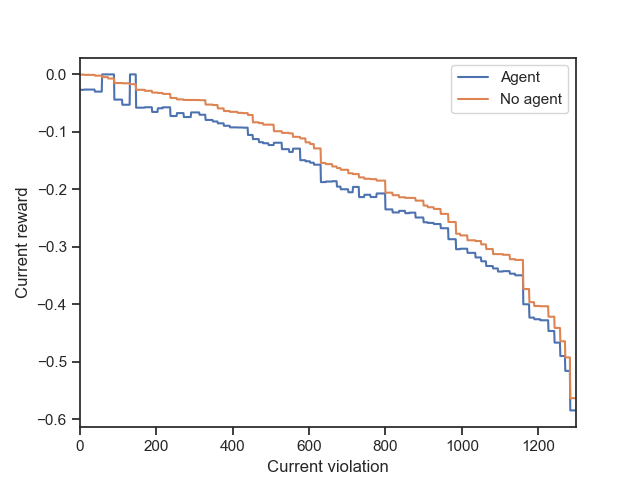
\includegraphics[height=8cm, width=12cm]{figures/config1_sorted_current.png}
    \caption[size = 9]{Current reward in critical hours sorted from best to worse for the trained agent and no agent scenario}
    \label{fig:results:config1_sorted_current}
\end{figure}

Figure \ref{fig:results:config1_improvement_current} shows hourly box plots for difference in current reward between the trained agent and the no agent scenario. This figure illustrates which hours of the day the agent performs best and worse. For current rewards, the trained agent is aggravating the situation in almost all hours. Hour 20 is the only time the agent improves the situation in terms of current magnitudes. Inspection of the hours with violations indicates that it is during noon (peak solar production) that the overloads happen, as illustrated in figure \ref{fig:results:config1_bad_current}.

\begin{figure}[h]
    \center
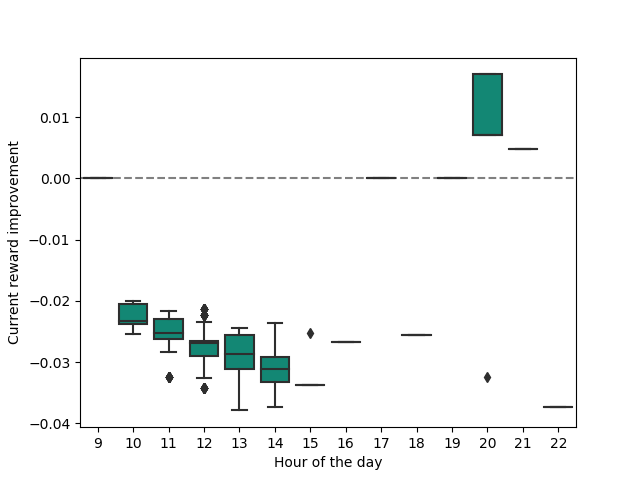
\includegraphics[height=8cm, width=12cm]{figures/config1_improvement_current.png}
    \caption[size = 9]{Hourly box plots of the difference in current rewards between the trained agent and no agent scenario in critical hours. Positive values means that the trained agent is better}
    \label{fig:results:config1_improvement_current}
\end{figure}



\begin{figure}[H]
    \center
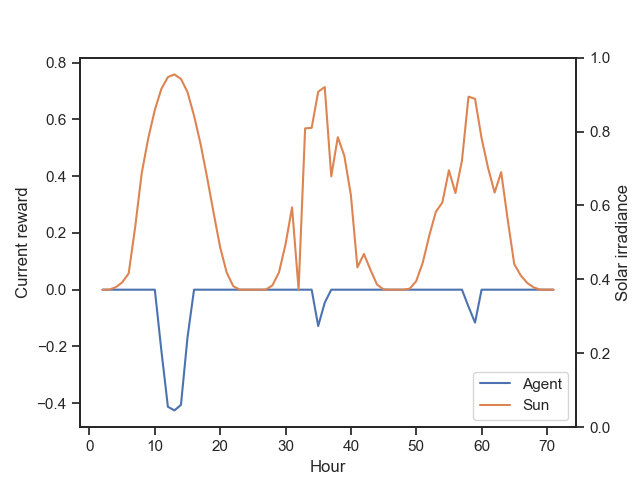
\includegraphics[height=8cm, width=12cm]{figures/config1_bad_current.png}
    \caption[size = 9]{Current reward and solar irradiance profile in a three day period. The agent is not able to prevent current overloads in hours of peak solar irradiance.}
    \label{fig:results:config1_bad_current}
\end{figure}


\subsection{Summary}
The trained agent shows a desired behaviour in terms of voltage magnitudes in periods of peak power demand. The power consumption is decreased in those periods, which keeps the voltage magnitudes above the lower safety margins. However, the trained agent has not found a strategy that keeps voltage magnitudes below upper margins in periods with peak solar production.

The agent performs poorly in terms of avoiding current overloads in the lines. This is only a problem in periods of peak solar production and not in hours of peak demand. There were no current overloads in the lines in hours of peek demand and the trained agent can consequently not be rated in that situation. The behaviour of the agent in the hours of peak demand and peak solar production is summarised in table \ref{table:results:config1_behaviour}.

\begin{table}[h]
\center
\begin{tabular}{l|ll}
                      & Current behaviour     & Voltage behaviour \\
\hline
Peak demand           & - & Good              \\
Peak solar production & Poor                  & Poor \\
\hline
\end{tabular}
\caption{Behaviour of the agent in critical periods in terms of current and voltage safety margins}
\label{table:results:config1_behaviour}
\end{table}
 A summary of the performance in terms of voltage and current is presented in table \ref{table:results:config1_summary}. Overall, the trained agent reduces the number of voltage and current violations by 10\%. However, it increases the mean cost by 5 \% due to its poor behaviour in terms of avoiding current violations. Still, the trained agent is better in terms of the total cost received in the 500 episode simulation because voltage violations are more frequent. The total cost in terms of both current and voltage is reduced by 3 \%.


\begin{table}[h]
\center
\begin{tabular}{l|lrrr}
Type      &               & Agent          & No agent       & Change        \\
\hline
Current   & Violations    & 1538            & 1300            & 18\%            \\
          & Mean cost     & 0,17           & 0,17           & 0 \%         \\
          & Cost          & 256            & 218            & 17 \%         \\
          &               &                &                &               \\
Voltage   & Violations    & 7484           & 8593           & -13\%          \\
          & Mean  cost    & 0,033          & 0,035          & -6\%          \\
          & Cost          & 249,9          & 304,5         & -18 \%        \\
          &               &                &                &               \\
Total     & Violations    & 9022           & 9893           & -10\%          \\
          & Mean cost     & 0.056          & 0.053          & 5 \%         \\
\textbf{} & \textbf{Cost} & \textbf{505.9} & \textbf{522.5} & \textbf{-3\%} \\
\hline
\end{tabular}
\caption{Summary of number of violations and mean costs in terms of current and voltage for the trained agent and the no agent scenario}
\label{table:results:config1_summary}
\end{table}

\end{document}